\documentclass[10pt]{article}
\usepackage[svgnames]{xcolor}
\usepackage{pgf,tikz}
\usepackage{mathrsfs}
\usetikzlibrary{arrows}
\pagestyle{empty}
\begin{document}
\definecolor{qqwuqq}{rgb}{0.,0.39215686274509803,0.}
\definecolor{ffxfqq}{rgb}{1.,0.4980392156862745,0.}
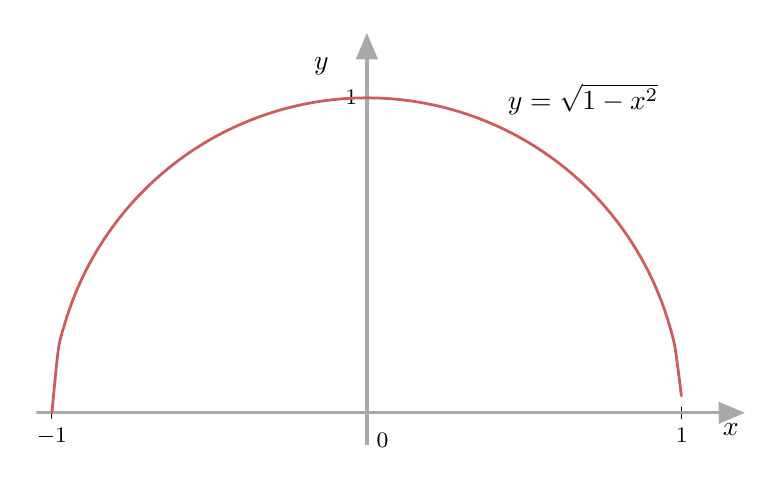
\begin{tikzpicture}[line cap=round,line join=round,>=triangle 45,x=4.0cm,y=4.0cm]
\foreach \x in {-1,1,}
\draw[shift={(\x,0)},color=black] (0pt,2pt) -- (0pt,-2pt) node[below] {\footnotesize $\x$};
\foreach \y in {1}
\draw[shift={(0,\y)},color=black]  node[left] {\footnotesize $\y$};
\draw[color=black] (0pt,-10pt) node[right] {\footnotesize $0$};
\clip(-1.049576759017141,-0.10010439784619256) rectangle (1.2204872478323576,1.2228591340144563);
\draw [->,line width=1.2pt,color=DarkGray] (-1.2,0.) -- (1.2,0.);
\draw [->,line width=1.2pt,color=DarkGray] (0.,-0.2) -- (0.,1.205870077907217);
\draw (1.3432939891865108,2.514190626435399) node[anchor=north west] {$y = \log \, (x-1)$};
\draw[line width=1.pt,color=IndianRed,smooth,samples=100,domain=-1:1] plot(\x,{sqrt(1.0-(\x)^(2.0))});
\draw (0.4166613044233548,1.0758631860299397) node[anchor=north west] {$y = \sqrt{1-x^{2}}$};
\draw (-0.09,1.1) node[left] {$y$};
\draw (1.0995412146805401,-0.003347571324738833) node[anchor=north west] {$x$};
\end{tikzpicture}
\end{document}